\chapter{Introducción a los grafos}
En este tema vamos a ver los diferentes tipos de grafos que existen para resolver problemas.
Veremos sobre los grafos (\textit{Dijkstra, Floyd, Warshall, Kruskal, Prim}, etc), donde cada uno tiene un proposito diferente, es decir, resuelven diferentes problemas y es importante saber cual resuelve cual a la hora de trabajar con ellos.

Para ello, primero vamos a ver que es un grafo y de que se compone.
\section{Definición de grafo}
Un \textbf{grafo} `G = (V,A)', consta de un conjunto de \textbf{vértices} o \textbf{nodos} (V) y de un conjunto de \textbf{aristas} o \textbf{arcos} (A) que define una relación banaria en V. Por tanto, podemos definir como que una arista es un par de vértices cualesquiera \((v,w) \in A\).

Si cada arista \((v,w) \in A\) es un par ordenado, es decir si, \((v,w)\) y \(w,v\) no son equivalentes, entonces el grado es \textbf{dirigido} y la arista resultante del par \((v,w)\) se representa con una \textit{flecha} indicando la dirección de \(v\) a \(w\) (\textit{Figura 8.1: Grafo dirigido}).
\begin{figure}[h]
  \begin{center}
    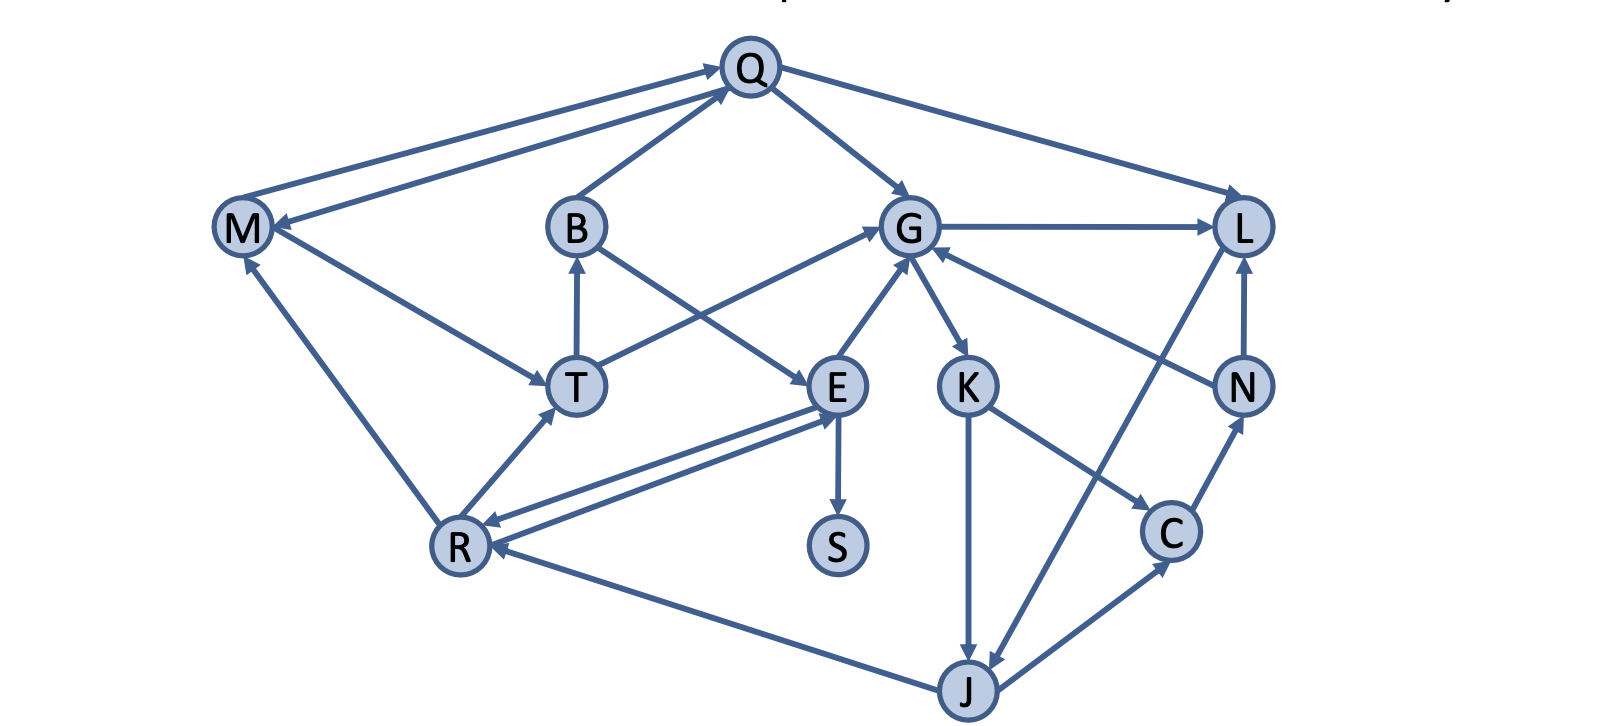
\includegraphics[width=.6\textwidth]{assets/intrografo1.png}
  \end{center}
  \caption{Grafo dirigido}
\end{figure}

\textit{NOTA: }Decimos que el vértice \(v\) es \textbf{incidente} sobre el vértice \(w\) y que \(w\) es \textbf{adyacente} a \(v\).

Por otro lado, si \((v,w)\) y \(w,v\) son \textbf{equivalentes} o \textbf{simétrico}, el grafo será \textbf{no dirigido}, y por tanto, la arista se representa como un \textit{segmento} entre \(v\) y \(w\), véase en la (\textit{Figura: 8.2 Grafo no dirigido}).

\begin{figure}[h]
  \begin{center}
    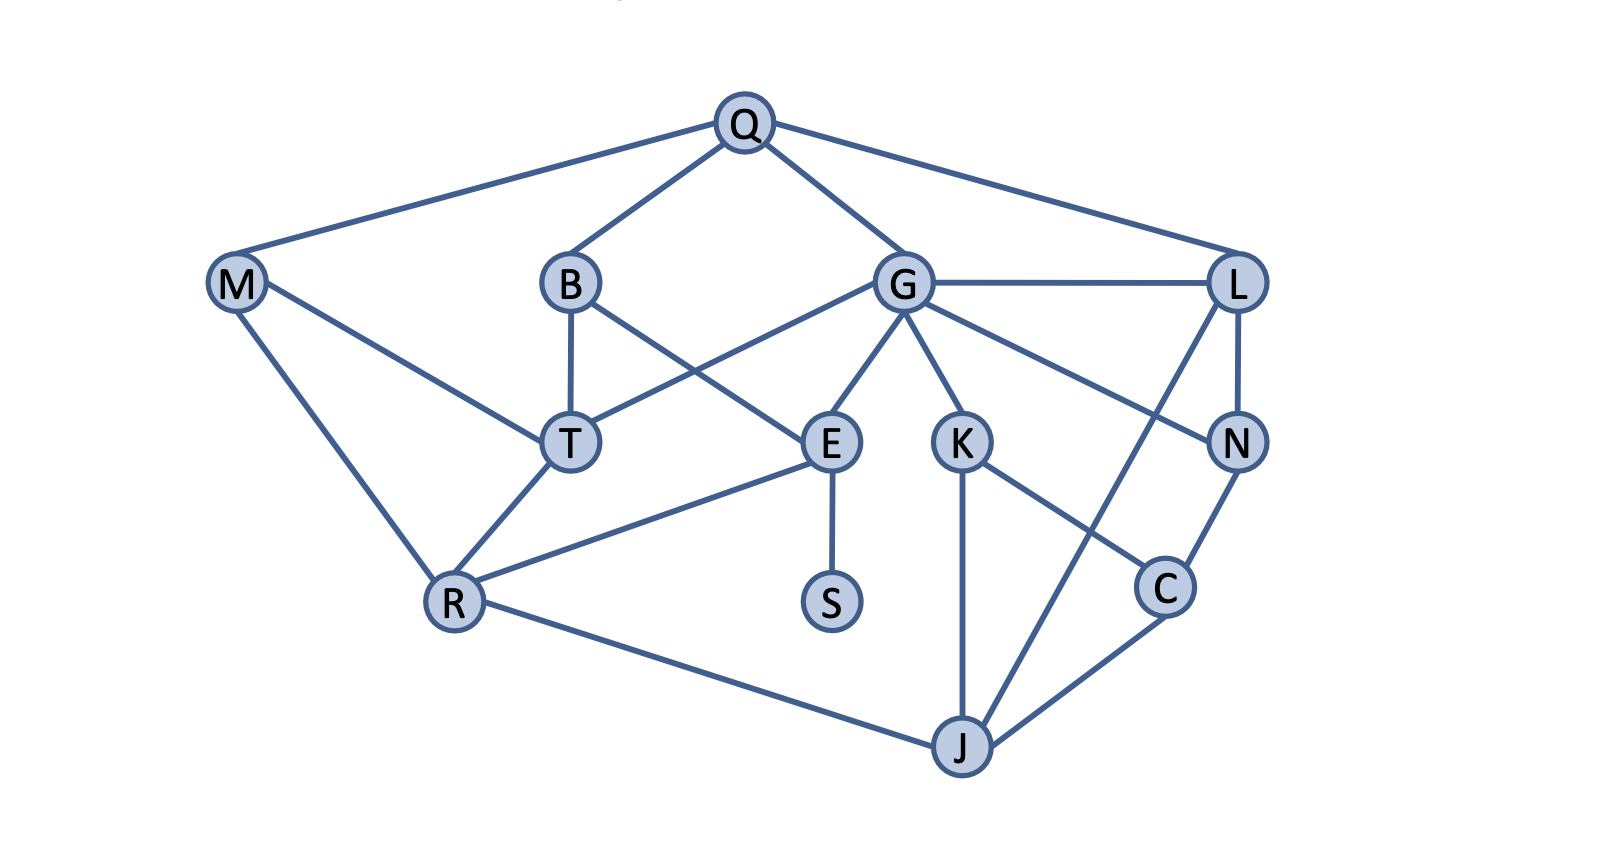
\includegraphics[width=.6\textwidth]{assets/intrografo2.png}
  \end{center}
  \caption{Grafo no dirigido}
\end{figure}

Cada arista del grafo puede tener asociada un valor asociado, llamado\textit{peso}, que indica el \textbf{coste} (tiempo, distancia, etc) de ir desde el vértice \(v\) al vértice \(w\). Un grafo el cual tenga un peso asociado a cada arista se le denomina \textbf{grafo ponderado}.
\begin{figure}[h]
  \begin{center}
    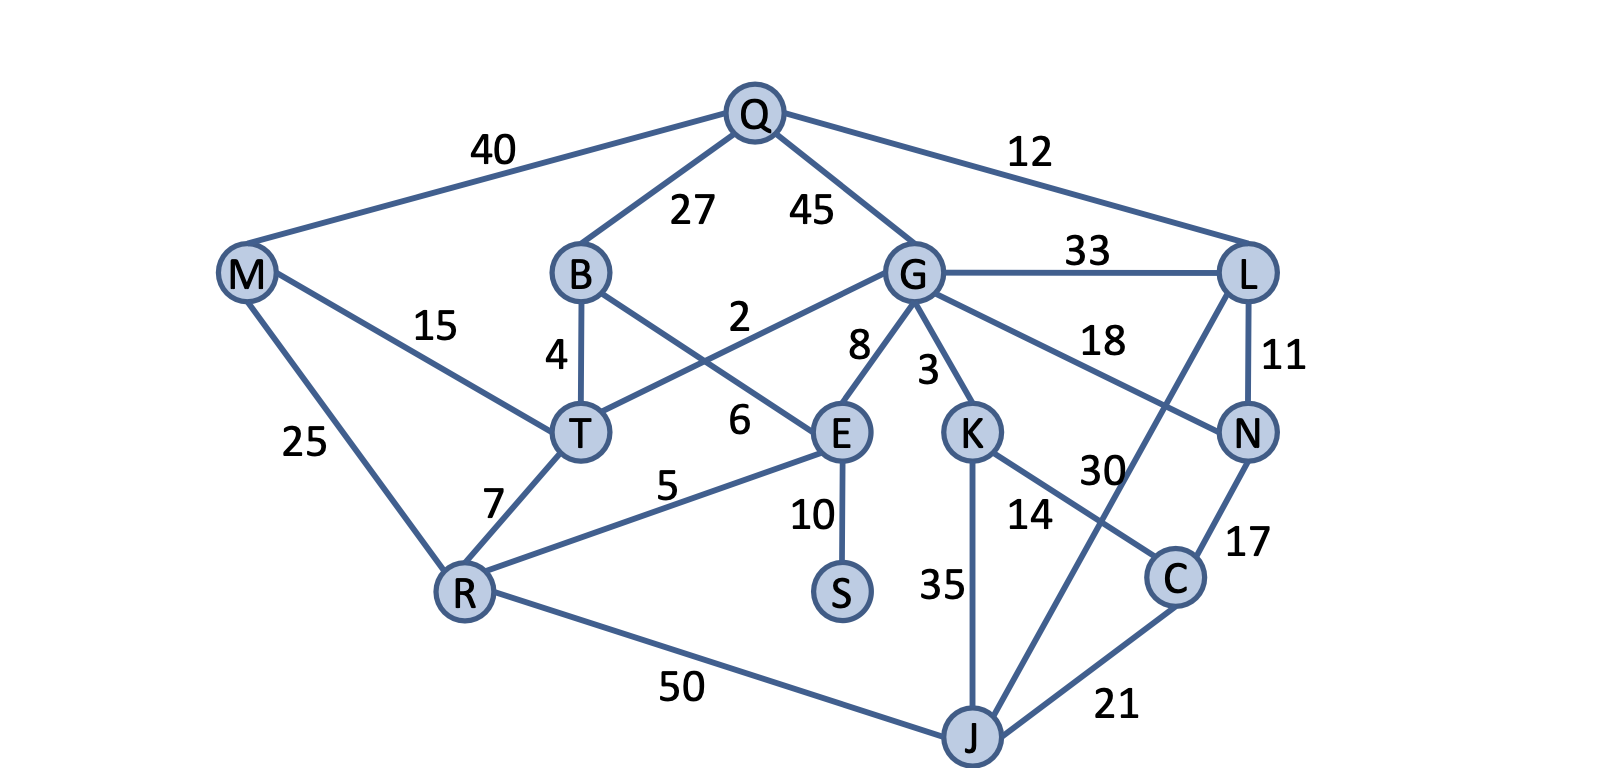
\includegraphics[width=.7\textwidth]{assets/intrografo3.png}
  \end{center}
  \caption{Grafo ponderado}
\end{figure}

\section{Definiciones }
Vamos a ver varias definiciones que debemos de saber cuando vayamos a trabajar con grafos.

\underbar{\large\textbf{Grado:}} El grado en un grafo no dirigido es el \textbf{número de arcos}. Si el grafo es dirigido se obtiene a partir de la diferencia entre \textbf{grado de entrada} y \textbf{grado de salida}, es decir, \(arcos\ incidentes - arcos\ adyacentes\).

\underbar{\large\textbf{Camino:}} Es una suceción de vértices de un grafo \(n_1, n_2,...,n_k\), tal que (\(n_i, n_{i+1}\)) es una arista para \(1\ \leq i\ < k\). La \textbf{longitud} del camino es el número de arcos que comprende, es decir \(k-1\), si el grafo no es ponderado. Si el grafo es ponderado, la longitud será la \textit{suma} de todos los pesos de las arista que lo componen.

\underbar{\large\textbf{Camino simple:}} Es el camino cuyos arcos son todos distintos, además si todos los vértices son distintos \(\rightarrow\) \textbf{camino elemental}.

\underbar{\large\textbf{Ciclo:}} Es el camino en el que coincide los vértices inicio y final. Si el camino es simple \(\rightarrow\) \textbf{ciclo simple} y si el camino es elemental \(\rightarrow\) \textbf{ciclo elemental}.

\underbar{\large\textbf{Grafo Conexo:}} Es un grafo \textbf{no dirigido} en el que al menos hay un camino entre cualquier par de vértice.
\begin{figure}[h]
  \begin{center}
    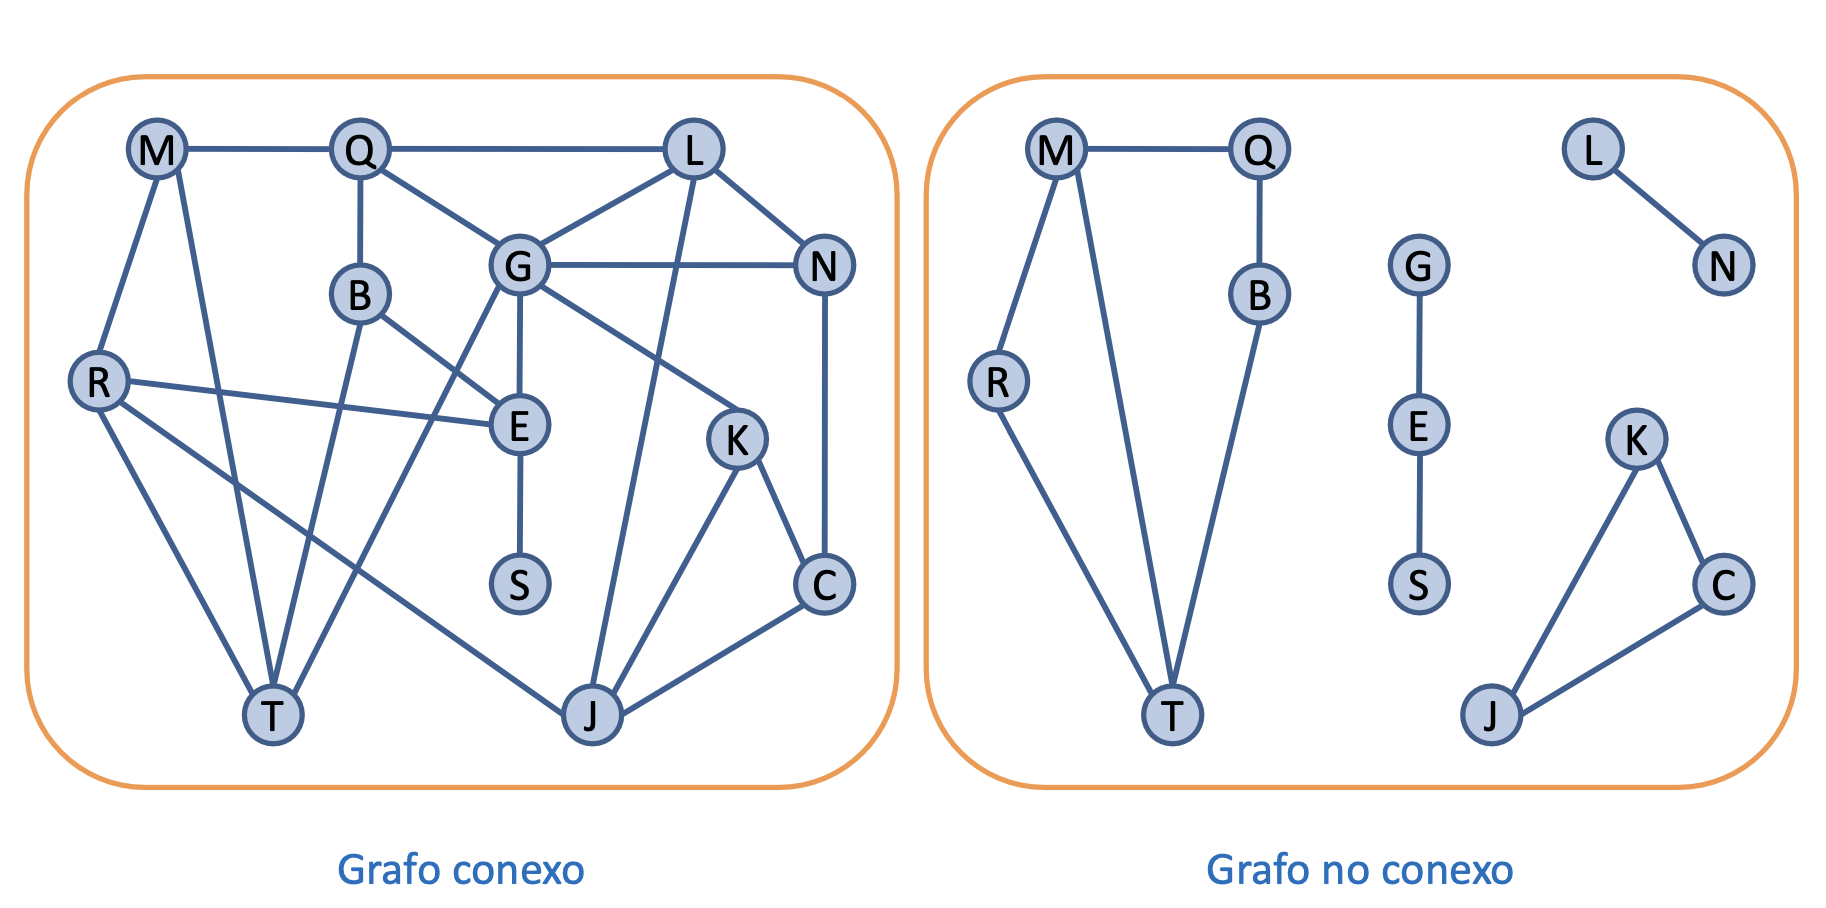
\includegraphics[width=.6\textwidth]{assets/intrografo4.png}
  \end{center}
  \caption{Diferencia entre grafo conexo y no conexo}
\end{figure}

\underbar{\large\textbf{Grafo fuertemente conexo:}} Es un grafo \textbf{dirigido} en el que hay la menos un camino entre cualquier par de vértices. Si un grafo dirigido no es fuertemente conexo, pero el grafo no dirigido \textit{subyacente} es conexo, diremos que el grafo es \textbf{débilmente conexo}.
\begin{figure}[h]
  \begin{center}
    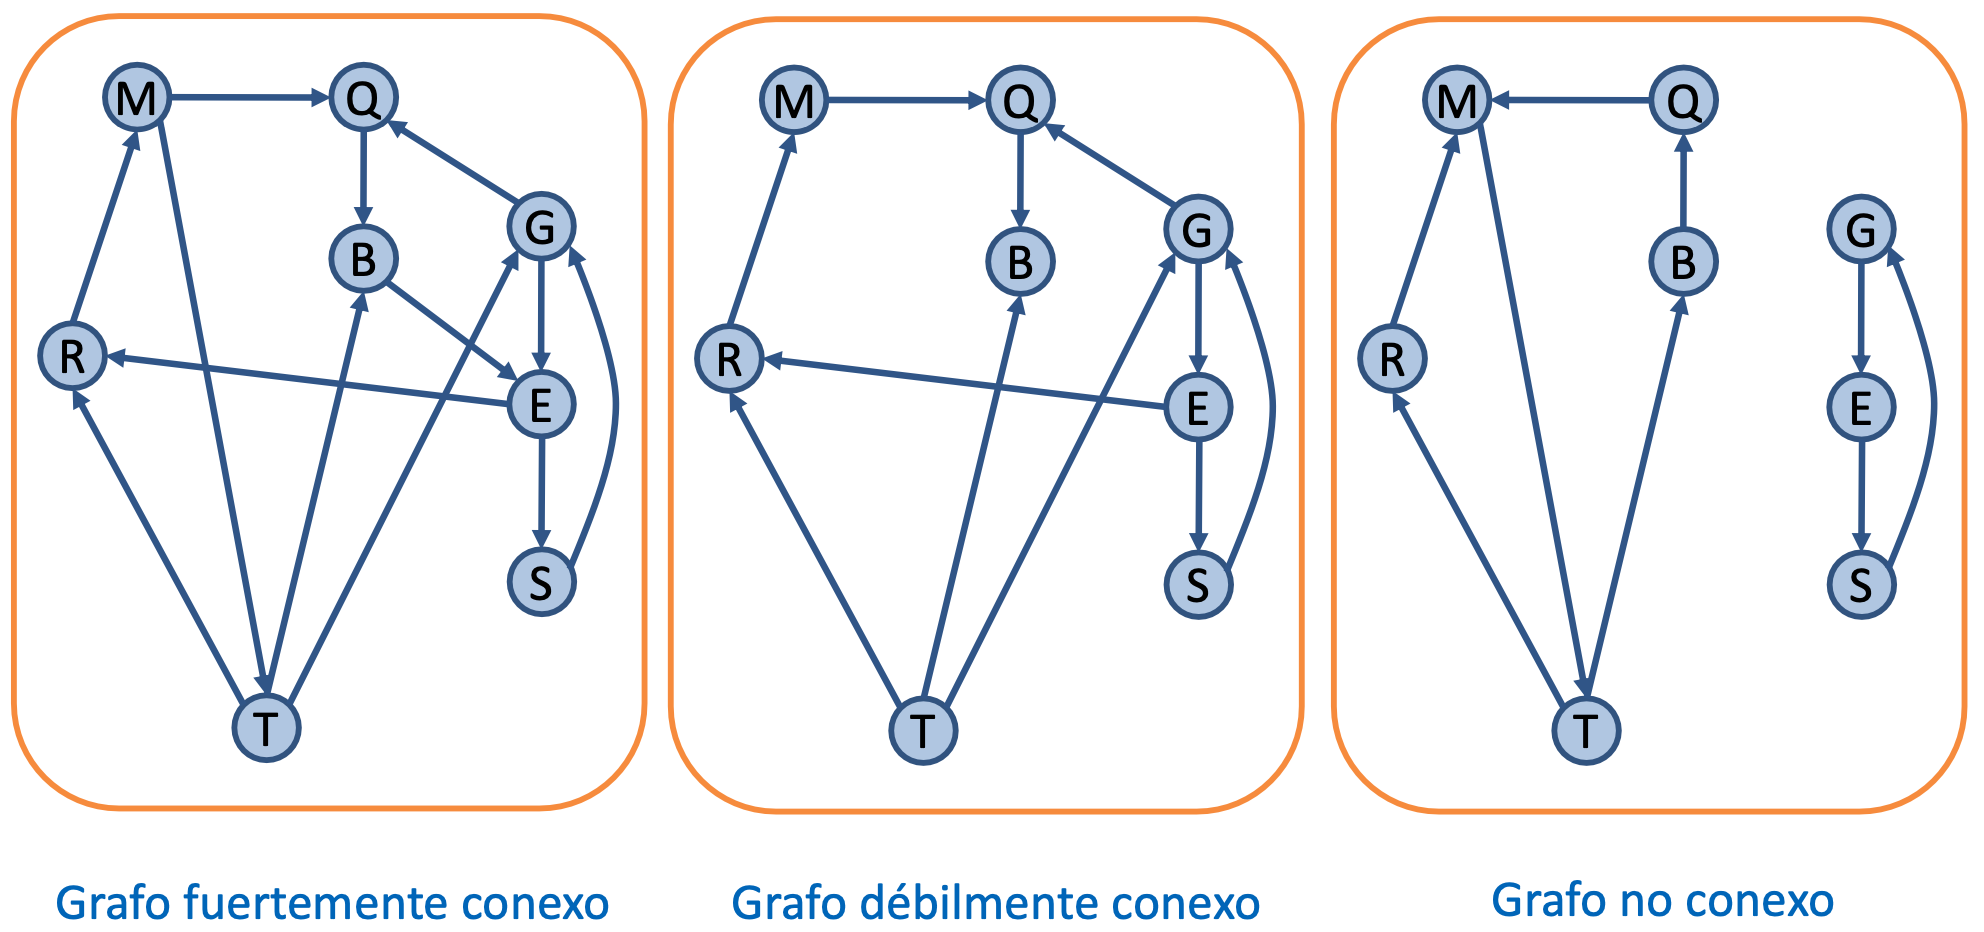
\includegraphics[width=.7\textwidth]{assets/intrografo5.png}
  \end{center}
  \caption{Ejemplos de grafos}
\end{figure}

\underbar{\large\textbf{Grafo completo:}} Es aquel que existe una arista entre cualquier par de vértices, si es en ambos sentido (segmento), es diremos que es completo y dirigido.
\begin{figure}[h]
  \begin{center}
    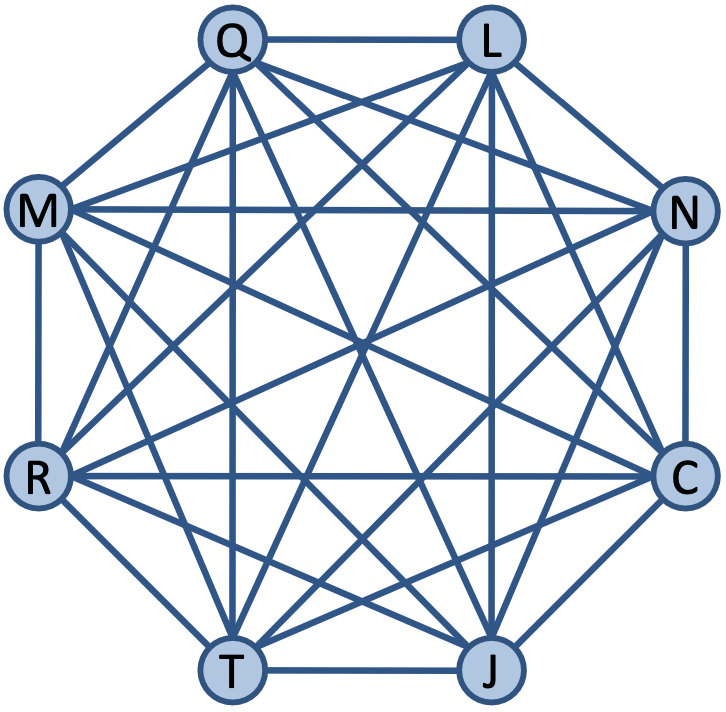
\includegraphics[width=.3\textwidth]{assets/intrografo6.png}
  \end{center}
  \caption{Ejemplos de grafo completo y dirigido}
\end{figure}

\underbar{\large\textbf{Subgrafo:}} Dado un grafo \(G = (V,A)\), diremos que el subgrafo \(G^` = (V^`,A^`)\) si \(A^`\) sólo contiene todas las aristas de \(A\) que unen los vértices de \(V^`\).

\section{Representaciones de grafos}
\begin{enumerate}
  \item \large\textbf{Matriz de adyacencia}
  
  Dado un grafo \(G = (V,A)\) con \(n\) vértices, se define la matriz de adyacencia asociada a \(G\) como una matriz \(M_{nxn}\), donde \(M_{i,j} = 1\) si \((i,j) \in A\) y \(M_{i,j} = 0\) si \((i,j) \notin A\).

  Si \(G\) es un grafo no dirigido, \(M\) será una matriz simétrica ya que \((i,j) =(j,i)\) para cualesquiera vértices i, j.

  \item \large\textbf{Matriz de costes}
  
  Dado un grafo \(G = (V,A)\) con \(n\) vértices, se define la matriz de coste asociada a \(G\) como una matriz \(C_{nxn}\), donde\\ \(Ci,j = p\) si \((i, j) \in A\), donde p = peso asociado a (i, j)\\
  \(Ci,j = peso\_ilegal\) si \((i, j) \notin A\), (peso\_ilegal = valor no válido como peso de un arco).
  Si no hay camino directo entre los dos vértices, se indicará con el valor \textbf{infinito}.
  \item \large\textbf{Listas de adyacencia}
  
  Asociamos a cada vértice \(i\) del grafo una lista que almacena todos los vértices adyacentes al mismo (\(i\)).
\end{enumerate}
\subsection*{Ventajas e inconvenientes}
\begin{itemize}
  \item Las \textbf{matrices de adyacencia} y \textbf{costes} son muy eficientes para comprobar si existe una arista entre dos vértices.
  \item Pueden desaprovechar una gran cantidad de memoria si el grafo no es completo.
  \item La representación mediante \textbf{listas de adyacencia} aprovechan mejor el espacio de memoria y son \textit{poco eficientes} para determinar si existe una arista entre dos vértices del grafo.
  \item Estas estructuras de datos \textbf{no admiten} la inserción y eliminación de vértices, pero la estructura \textbf{lista de listas de adyacencia} si se permite la adición y eliminación de vértices.
\end{itemize}
